\chapter{Design\label{cha:chapter4}}

In this chapter, I will detail the design of the implemented testbed shown in \Cref{fig:testbed}. 

\section{Producer\label{sec:producer}}

The Producer is a highly configurable Rust program capable of reading special settings-files with which a FFmpeg \footnote{FFmpeg Homepage: \url{https://www.ffmpeg.org/}} command is generated. FFmpeg is a powerful command line tool for audio and video processing.

The generation process starts with the parsing of the CLI, specifics follow in \Cref{sec:cli_producer}, followed by the reading of the settings files, according to \Cref{sec:settings}. Using the parameters gathered from the CLI and settings-files, the Producer generates a shell scripts. The Producer supports a plethora of input types, see \Cref{sec:producer_inputs} for full details. 

When a local video file is configured as the input, the FFmpeg command will create a live stream by looping through the video endlessly. Video devices usually represent the built-in laptop webcam, but it is also possible to plug in an external camera via USB and use that as an input, the setup process is described in the following \Cref{sec:ext_cam}. Remote video sources can be anything supported by FFmpeg that can be addressed using an URL, for example remotely hosted DASH/HLS live streams or VoDs (videos on demand) or IP-cameras.

Once the Producer has finished generating the FFmpeg shell script, the script can be executed in a terminal to run the live stream creation. The FFmpeg command will create the live stream using the output format "dash" and point the output to an HTTP server. The "dash" output format also has a convenient option to create HLS master and media playlist files alongside the DASH stream. 

An example shell scripts is shown in \Cref{ex:shell}.

\subsection{Command Line Interface\label{sec:cli_producer}}

As previously mentioned, the Command Line Interface (CLI) of the Producer has many options to configure it for many different use-cases. The Producer is primarily intended to create DASH live streams, which is why the output flag must point to a DASH Manifest MPD file with either a local path or an URL. The audio and video settings flags are optional and when not provided, the Producer will automatically generate the settings files and re-use them on subsequent uses.

To simplify the usage of these complex options, I have created a helper script to easily use the Producer with a few pre-configured methods during development, details will follow in \Cref{sec:docu}.

\begin{table}[H]
    \centering
    \begin{tabular}{|r|r|l|l|}
    \hline
    \multicolumn{1}{|l|}{\textbf{Short Flag}} & \multicolumn{1}{l|}{\textbf{Long Flag}} & \textbf{Value}                                      & \textbf{Description}                                                                        \\ \hline
    -o                                        & --output                                & \begin{tabular}[c]{@{}l@{}}Path/\\ URL\end{tabular} & \begin{tabular}[c]{@{}l@{}}The path to the output\\ DASH Manifest file (*.mpd)\end{tabular} \\ \hline
    -a                                        & --audio                                 & Path                                                & \begin{tabular}[c]{@{}l@{}}The path to the audio\\ settings file\end{tabular}               \\ \hline
    -v                                        & --video                                 & Path                                                & \begin{tabular}[c]{@{}l@{}}The path to the video\\ settings file\end{tabular}               \\ \hline
    -s                                        & --script                                & Path                                                & \begin{tabular}[c]{@{}l@{}}The path to the script\\ file to create\end{tabular}             \\ \hline
                                              & --ll                                    & boolean                                             & Enable Low Latency                                                                          \\ \hline
    -t                                        & --title                                 & String                                              & Set the title of the stream                                                                 \\ \hline
                                              & --hls                                   & boolean                                             & \begin{tabular}[c]{@{}l@{}}Enable concurrent HLS\\ Manifest creation\end{tabular}           \\ \hline
                                              & --an                                    & boolean                                             & Disable audio                                                                               \\ \hline
                                              & --vn                                    & boolean                                             & Disable video                                                                               \\ \hline
    -k                                        & --keyframes                             & u8                                                  & \begin{tabular}[c]{@{}l@{}}Number of keyframes \\ per Fragment\end{tabular}                 \\ \hline
                                              & --fps                                   & f32                                                 & Frame per second                                                                            \\ \hline
                                              & --segdur                                & f32                                                 & \begin{tabular}[c]{@{}l@{}}Target Fragment\\ Duration\end{tabular}                          \\ \hline
                                              & --embed-settings                        & boolean                                             & \begin{tabular}[c]{@{}l@{}}Embed selected encoding\\ settings into the video\end{tabular}   \\ \hline
    \end{tabular}
    \caption{Producer CLI Options}
\end{table}

The input of the live stream is configured using a subcommand of the Producer. I will give each type of input its own section.

\subsubsection{Remote}

The \textbf{remote} command uses an external resource as input. Anything that can be addressed using an URL and that is natively supported by FFmpeg can be used. For example publicly hosted DASH / HLS streams, IP-cameras or more.

The only option this command has is a positional argument pointing to the remote input in form of an URL.

\subsubsection{Local}

The \textbf{local} command takes a local file as input. This is essentially the same as the remote command, the difference being that it uses an local path instead of a remote URL. The same restrictions apply.

The path is supplied with a positional argument. However, it has a second option. This being whether or not to create a live stream. For example, when using a video file as input, this video has a finite runtime. Setting this flag will make FFmpeg loop through the file endlessly to create a live stream.

\begin{table}[H]
    \centering
    \begin{tabular}{|r|r|l|l|}
    \hline
    \multicolumn{1}{|l|}{\textbf{Short Flag}} & \multicolumn{1}{l|}{\textbf{Long Flag}} & \textbf{Value} & \textbf{Description}                                                   \\ \hline
                                              &                                         & Path           & \begin{tabular}[c]{@{}l@{}}The path to the input\\ file.\end{tabular}  \\ \hline
    -l                                        & --live                                  & boolean        & \begin{tabular}[c]{@{}l@{}}Loop through the \\ video file\end{tabular} \\ \hline
    \end{tabular}
    \caption{Local Command Options}
\end{table}

\subsubsection{Standard Input Pipe}

The \textbf{std-in} command uses the standard input pipe to receive raw video data as input for FFmpeg.

The only required option is the resolution of the video data, given with the height and width of the video in number of pixels.

\begin{table}[H]
    \centering
    \begin{tabular}{|r|r|l|l|}
    \hline
    \multicolumn{1}{|l|}{\textbf{Short Flag}} & \multicolumn{1}{l|}{\textbf{Long Flag}} & \textbf{Value} & \textbf{Description} \\ \hline
                                              & --w                                     & u16            & The pixel width      \\ \hline
                                              & --h                                     & u16            & The pixel height     \\ \hline
    \end{tabular}
    \caption{Standard Input Command Options}
\end{table}

\subsubsection{Device}

The \textbf{device} command uses a capture device as input. The most common use-case for this would be the webcam of a laptop. On Linux, device are addressed using a path to the device directory (\texttt{/dev/*}), for example the built-in webcam of a laptop is typically the \texttt{/dev/video0} device, which this command defaults to.

As before, the path is given as argument with the additional option to set which input format to use.

\begin{table}[H]
    \centering
    \begin{tabular}{|r|r|l|l|}
    \hline
    \multicolumn{1}{|l|}{\textbf{Short Flag}} & \multicolumn{1}{l|}{\textbf{Long Flag}} & \textbf{Value} & \textbf{Description}                                                      \\ \hline
                                              &                                         & Path           & \begin{tabular}[c]{@{}l@{}}The path to the \\ capture device\end{tabular} \\ \hline
    -f                                        & --format                                & String         & Input format                                                              \\ \hline
    \end{tabular}
    \caption{Device Command Options}
\end{table}

\subsubsection{Screen}

The \textbf{screen} command uses the device's screen as input. I have not fully developed this command to be completely usable, since this turned out to be more complex than I initially expected it to be and I needed to focus on more important aspects. The original intention was to have it work similar to other screen capture tools where the user can select a specific window, screen or sub-region of a screen with a resolution and capture frame rate to create a live screen.

\subsubsection{Test}

The \textbf{test} command is the final input method. It uses the built-in FFmpeg virtual input format \texttt{lavfi} to generate a test image. This test image has a few vertical colorful bars, a horizontal scrolling gradient with a timestamp counting up the seconds the has been stream running for. Examples for this test image can be seen in \Cref{fig:incomple_mt}, \Cref{fig:merkle_tree} and \Cref{fig:rolling_hash}.

This input can be configured with a starting resolution, frame rate and an optional duration of the generated video. If the duration is omitted, it will create an endless stream. Otherwise, the duration is provided in milliseconds.

\begin{table}[H]
    \centering
    \begin{tabular}{|r|r|l|l|}
    \hline
    \multicolumn{1}{|l|}{\textbf{Short Flag}} & \multicolumn{1}{l|}{\textbf{Long Flag}} & \textbf{Value} & \textbf{Description}                                                        \\ \hline
                                              & --w                                     & u16            & The pixel width                                                             \\ \hline
                                              & --h                                     & u16            & \begin{tabular}[c]{@{}l@{}}Loop through the \\ video file\end{tabular}      \\ \hline
    -r                                        & --fps                                   & f32            & Input frame rate                                                            \\ \hline
    -d                                        & --dur                                   & u64            & \begin{tabular}[c]{@{}l@{}}Optional duration\\ in milliseconds\end{tabular} \\ \hline
    \end{tabular}
    \caption{Test Command Options}
\end{table}

\subsection{Settings Files\label{sec:settings}}

The settings files are two CSV-files, one for audio and video each. These files are automatically generated the first time the Producer is run. The initial default configurations are shown in \Cref{list:audio} for audio and video in \Cref{list:video} (both are formatted for better readability). These files can be configured by adding new lines with desired settings or by removing lines with unwanted settings, alternatively they can also be made to be ignored by Producer by adding a '\texttt{\#}' in front of a line.

\begin{figure}
    \centering
    \begin{lstlisting}
           name,sampling,bitrate
        default,   48000, 128000
    \end{lstlisting}
    \caption{Default Audio Settings File}
    \label{list:audio}
\end{figure}

\begin{figure}
    \centering
    \begin{lstlisting}
          name,resolution, bitrate,max_rate,buffer_size
         #144p,   256x144,   95000,  100000,     150000
         #240p,   426x240,  150000,  160000,     240000
         #360p,   640x360,  276000,  290000,     430000
         #480p,   854x480,  750000,  775000,    1200000
          720p,  1280x720, 2048000, 2200000,    3300000
        #1080p, 1920x1080, 4096000, 4300000,    6500000
        #1440p, 2560x1440, 6144000, 6500000,   10000000
        #2160p, 3840x2160,17408000,18000000,   27000000
    \end{lstlisting}
    \caption{Default Video Settings File}
    \label{list:video}
\end{figure}

\section{Signer\label{sec:signer}}

The Signer is an extension of the existing \texttt{c2patool} command line program and the underlying \texttt{c2pa-rs} Rust crate. It has been extended by an additional subcommand to run the tool in live signing mode, alongside the implementation of signing processes optimized for live streaming purposes. The live subcommand turns the \texttt{c2patool} into an HTTP server. The Signer will then receive the live stream from FFmpeg via HTTP requests. With every new fragment received the stream will be signed, details of the signing and the optimizations are detailed in \Cref{sec:optimization} and the alternative approach is presented in \Cref{sec:rolling_hash}. Finally, the finished files are then sent to the Distributor.

\subsection{Command Line Interface\label{sec:cli_signer}}

The CLI of the Signer, which is actually the \texttt{c2patool} is quite extensive. In an effort to keep it concise and not too complex, I will only list the options that I am using in this testbed and those, I have added to implement live signing.

As before, I will begin with the general options. The path to the asset file is an argument, making it not require any designating flag. In normal operation, this file is the target of either signing or validation. However, since my live signing approach uses an HTTP server to receive files, I have no use for this argument. But since this argument is mandatory, I simply pass it arbitrary data and ignore it.

\begin{table}[H]
    \centering
    \begin{tabular}{|r|r|l|l|}
    \hline
    \multicolumn{1}{|l|}{\textbf{Short Flag}} & \multicolumn{1}{l|}{\textbf{Long Flag}} & \textbf{Value} & \textbf{Description}                                                                \\ \hline
                                              &                                         & Path           & The path to the asset file.                                                         \\ \hline
    -o                                        & --output                                & Path           & \begin{tabular}[c]{@{}l@{}}The path to the output\\ file or directory\end{tabular} \\ \hline
    -m                                        & --manifest                              & Path           & \begin{tabular}[c]{@{}l@{}}The path to the C2PA\\ Manifest JSON file\end{tabular} \\ \hline
    \end{tabular}
    \caption{Signer CLI Options}
\end{table}

In addition to the general options the \texttt{c2patool} uses a few commands for additional configuration. As previously mentioned, I have added the "live" command to the tool. This command turns the \texttt{c2patool} into an HTTP server to receive the live stream from the Producer. The target URL is the ingestion URL of the CDN.

\begin{table}[H]
    \centering
    \begin{tabular}{|r|r|l|l|}
    \hline
    \multicolumn{1}{|l|}{\textbf{Short Flag}} & \multicolumn{1}{l|}{\textbf{Long Flag}} & \textbf{Value}                                           & \textbf{Description}                                                                              \\ \hline
    -b                                        & --bind                                  & \begin{tabular}[c]{@{}l@{}}Socket\\ Address\end{tabular} & \begin{tabular}[c]{@{}l@{}}The Socket Address on which \\ the Signer will listen on.\end{tabular} \\ \hline
    -t                                        & --target                                & URL                                                      & \begin{tabular}[c]{@{}l@{}}The CDN URL where to\\ ingest the output to\end{tabular}              \\ \hline
    -w                                        & --window                                & usize                                                    & \begin{tabular}[c]{@{}l@{}}The number of Fragment\\ in one Merkle Tree group\end{tabular}        \\ \hline
    \end{tabular}
    \caption{Live Command Options}
\end{table}

\subsection{Signing Approaches\label{sec:rolling_hash}}

As explained in \Cref{sec:sign_bmff}, the existing fragment BMFF signing implementation is designed to be used to sign a completed set of files, i.e. a VoD. As a preliminary experiment, I used this implementation to sign the created live stream in this testbed to see how it works. This approach does actually work and the fragments are all correctly validated. However, since this implementation always signs all files given to it, with every newly generated fragment, the entire live stream is signed anew. This caused the signing to take longer and longer with every fragment, continuously slowing down the machine it is running on and eventually it could no longer keep up and the live stream would begin to stall. Additionally, after every signing operation all fragments needed to published again to the CDN, which created a lot of overhead on the network and CDN, while also not letting the CDN effectively cache the fragments. I included this approach in my evaluation of this thesis to better show the effectiveness of my optimized implementations.

Next, I started the implementation of the optimized signing processes. I began with an optimized Merkle Tree approach as per the original proposal and the other alternatives were created in response to some of the drawbacks of the Merkle Tree approach.

\subsubsection{Optimized Merkle Tree}

As mentioned, the big problem with the existing Merkle Tree approach was the complete re-signing of files that had already been signed during a previous signing. To fix this problem, I made use of the fact that the C2PA Manifest is able to hold multiple Merkle Trees, as shown in \Cref{sec:bmff_assertion}. Each Merkle Tree has a unique and local ID and each fragment's embedded data has these IDs as well, which are used to assign a fragment to the matching Merkle Tree.

This approach required the addition of a new parameter to the signing function: the window size. This window size corresponds to the number of fragments each Merkle Tree will hold at most. The window size can be configured using the CLI of the Signer as depicted in \Cref{sec:cli_signer}, for the duration of this thesis, I have used a window size of \texttt{8} as the default value. I chose this value for a number of reasons. Firstly, since a Merkle Tree is a binary tree it is a good idea to use a power of two value to completely fill all layers of a tree. Secondly, I figured that \texttt{8} strikes a decent balance between having enough fragments grouped together for security, while not having so many fragments that signing would take too much time.

This way only requires to sign the newest up to \texttt{8} (or window size) fragments of the live stream. Once a full group of \texttt{8} fragments has been signed, they are done and no longer need to be updated on the CDN. This approach greatly improved the performance of the live stream signing, however, it still came with a number of drawbacks:

\begin{itemize}
    \item each group of fragments adds another Merkle Tree to the BMFF Hash Assertion in the C2PA Manifest, this could result in the C2PA Manifest becoming too big if the Live Stream runs for a very long time
    \item each fragment still has to be updated on the CDN up to \texttt{8} times
    \item the initialization fragment still needs to be updated every time a new fragment is created
    \item validation of every fragment requires the fetching of the newest initialization fragment to have the corresponding C2PA Manifest
    \item a live stream could be tampered with by replacing a full group of a Merkle Tree
\end{itemize}

The technical details of this approach are described in \Cref{sec:merkle_opt}.

The next two approaches are extensions of this method and were created in response to the frequent uploading and downloading of essentially the same fragments.

\subsubsection{Optimized Merkle Tree with C2PA Data on separate Server}

In this approach, the C2PA data added to the fragments by the signing process are stored on a separate server. First, the unsigned fragments that come in from the Producer are embedded with a "uuid" BMFF Box, which contains only the URL to the C2PA data on the separate server. The fragments are then published to the CDN. These fragments never change and this allows the CDN to work as they would in a non-C2PA scenario.

Now only the C2PA data needs to be updated on the server, which are significantly smaller than the media fragments.

The validation has the added steps of reading the URL in the "uuid" box in the fragments, downloading the data from that URL, replacing the "uuid" box with the downloaded data. Then the fragment can be validated as before.

The big drawback of the approach is the introduction of an additional attack vector, being the extra server.

The technical details and issues with this approach follow in \Cref{sec:on_server}.

\subsubsection{Optimized Merkle Tree with C2PA Data in DASH/HLS Manifests}

This approach is very similar to the previous one with the C2PA data being kept separate from the actual fragments. However, in this approach, the C2PA data is written in to the Manifests of the DASH and HLS protocols, specifically the MPD for DASH and the MediaPlaylist of HLS.

An advantage of this is the fact that in a typical live streaming scenario it is very common that the Manifests are updated and downloaded on a per fragment-basis anyways. This way the C2PA data is essentially received for free, barring some bigger Manifests.

One problem with this approach is adding the data to the Manifests. Initially, I started by forking the respective parsing crates to simply add new data fields to the Manifests, which would have no longer been conform to their respective specifications. I would have needed to do the same for the client as well to read out the new data again and that started to become too complex. An alternative could be to misuse an existing field for this purpose. For example event-signaling could be abused for this purpose, similar to ad-insertion.

The technical details and issues with this approach follow in \Cref{sec:in_manifest}.

\subsubsection{Rolling Hash Approach}

With the knowledge I gathered from the three previous approaches, I came up with a completely new approach, which attempts to deal with as many of the drawbacks of those approaches.

The notable change is the replacement of the Merkle Tree with a Rolling Hash. This is done through an extension of the BMFF Hash Assertion. This extension holds most notably the Rolling Hash, as well as the Anchor Point. The fragments themselves only contain the Anchor Point.

This new signing function only needs the initialization fragment and the new fragment to be sign. If the new fragment is the first fragment of the live stream, then the C2PA Manifest is embedded into the initialization fragment and the Rolling Hash is the hash of the hash of the fragment. The Anchor Point is empty. All the following fragments will use the Rolling Hash of the previous fragment as their Anchor Point (saved in the fragment and the C2PA Manifest) and create the new Rolling Hash by hashing the concatenation of the Anchor Point + hash of the fragment.

The initialization fragment still needs to be updated with each new fragment, however, each fragment only needs to be published once.

The validation begins as before by validating the initialization fragment and the validation of fragments depends on whether the starting fragment is the first fragment of the live stream or any other fragment. 

If it is the very first fragment, validation is very simple and only needs to hash the hash of the fragment and compare it with the Rolling Hash found in the C2PA Manifest of the initialization fragment. The resulting Rolling Hash can then be stored and used as Anchor Point for the next fragment: hash the next fragment and create the Rolling Hash as above through concatenation.

When the starting fragment was not the first fragment in the live stream, validation adds one more step. Extracting the Anchor Point from the fragment itself and comparing it with the Anchor Point found in the C2PA Manifest. From here validation continues as above.

This approach also makes use of the EventStream in the DASH MPD to embed the Anchor Points and Rolling Hash of the C2PA Manifest from the initialization fragment. This way, the client only needs to download the initialization fragment with the contained C2PA Manifest once and then it receives the new Rolling Hash and Anchor Point from the MPD.

This approach fixes most of the problems of the other approaches:

\begin{itemize}
    \item Rolling Hash doesn't make the C2PA Manifest grow over time
    \item fragments only need to be published once
    \item validation doesn't need to download any additional data, uses data from the MPD
    \item parts of the live stream can no longer be replaced, because that would break the Rolling Hash
    \item no additional attack vector is added
    \item it remains specification conform (to DASH and HLS, not C2PA)
\end{itemize}

However, there still remain some drawbacks:

\begin{itemize}
    \item the initialization fragment still needs to be updated with every new fragment
    \item fragments can only be validated if the full Rolling Hash up to the newest fragment is created
\end{itemize}

\section{Distributor\label{sec:cdn}}

The signed live stream is hosted on a CDN. A CDN is an HTTP server, which can receive data and then distribute it using HTTP requests. The CDN receives the live stream from the Signer and then distributes it to the Consumer.

The CDN caches all new files in memory to ensure that they can be provided as fast as possible. The files are cleared from the cache when FFmpeg signals their removal. The technical details follow in \Cref{sec:caching}.

\subsection{Command Line Interface\label{sec:cli_cdn}}

The CLI of the CDN is kept rudimentary, since it doesn't require much configuration. 

\begin{table}[H]
    \centering
    \begin{tabular}{|r|r|l|l|l|}
    \hline
    \textbf{Short Flag} & \textbf{Long Flag} & \textbf{Value}                                            & \textbf{Description}                                                                           & \textbf{Default} \\ \hline
    -b                  & --bind             & \begin{tabular}[c]{@{}l@{}}Socket \\ Address\end{tabular} & \begin{tabular}[c]{@{}l@{}}The Socket Address on \\ which the CDN will listen on\end{tabular} & {[}::{]}:6363    \\ \hline
    -m                  & --media            & Path                                                      & \begin{tabular}[c]{@{}l@{}}The Path to the Directory \\ where to write Data to\end{tabular}   & ./media          \\ \hline
    \end{tabular}
    \caption{CDN CLI Options}
\end{table}                                                      

\section{Consumer\label{sec:consumer}}

The Consumer is a website built using the SvelteKit \footnote{Svelte Homepage: \url{https://svelte.dev/}} framework. The website consists of four major parts: Controls, Player, Manifest and the Visualization of either the Merkle Tree or the Rolling Hash. \Cref{fig:merkle_tree} shows an example of the visualization of a full Merkle Tree and a similar example of a Rolling Hash is shown in \Cref{fig:rolling_hash}. In the appendix there is also an example image of an incomplete Merkle Tree, see \Cref{fig:incomple_mt}.

\begin{figure}
    \centering
    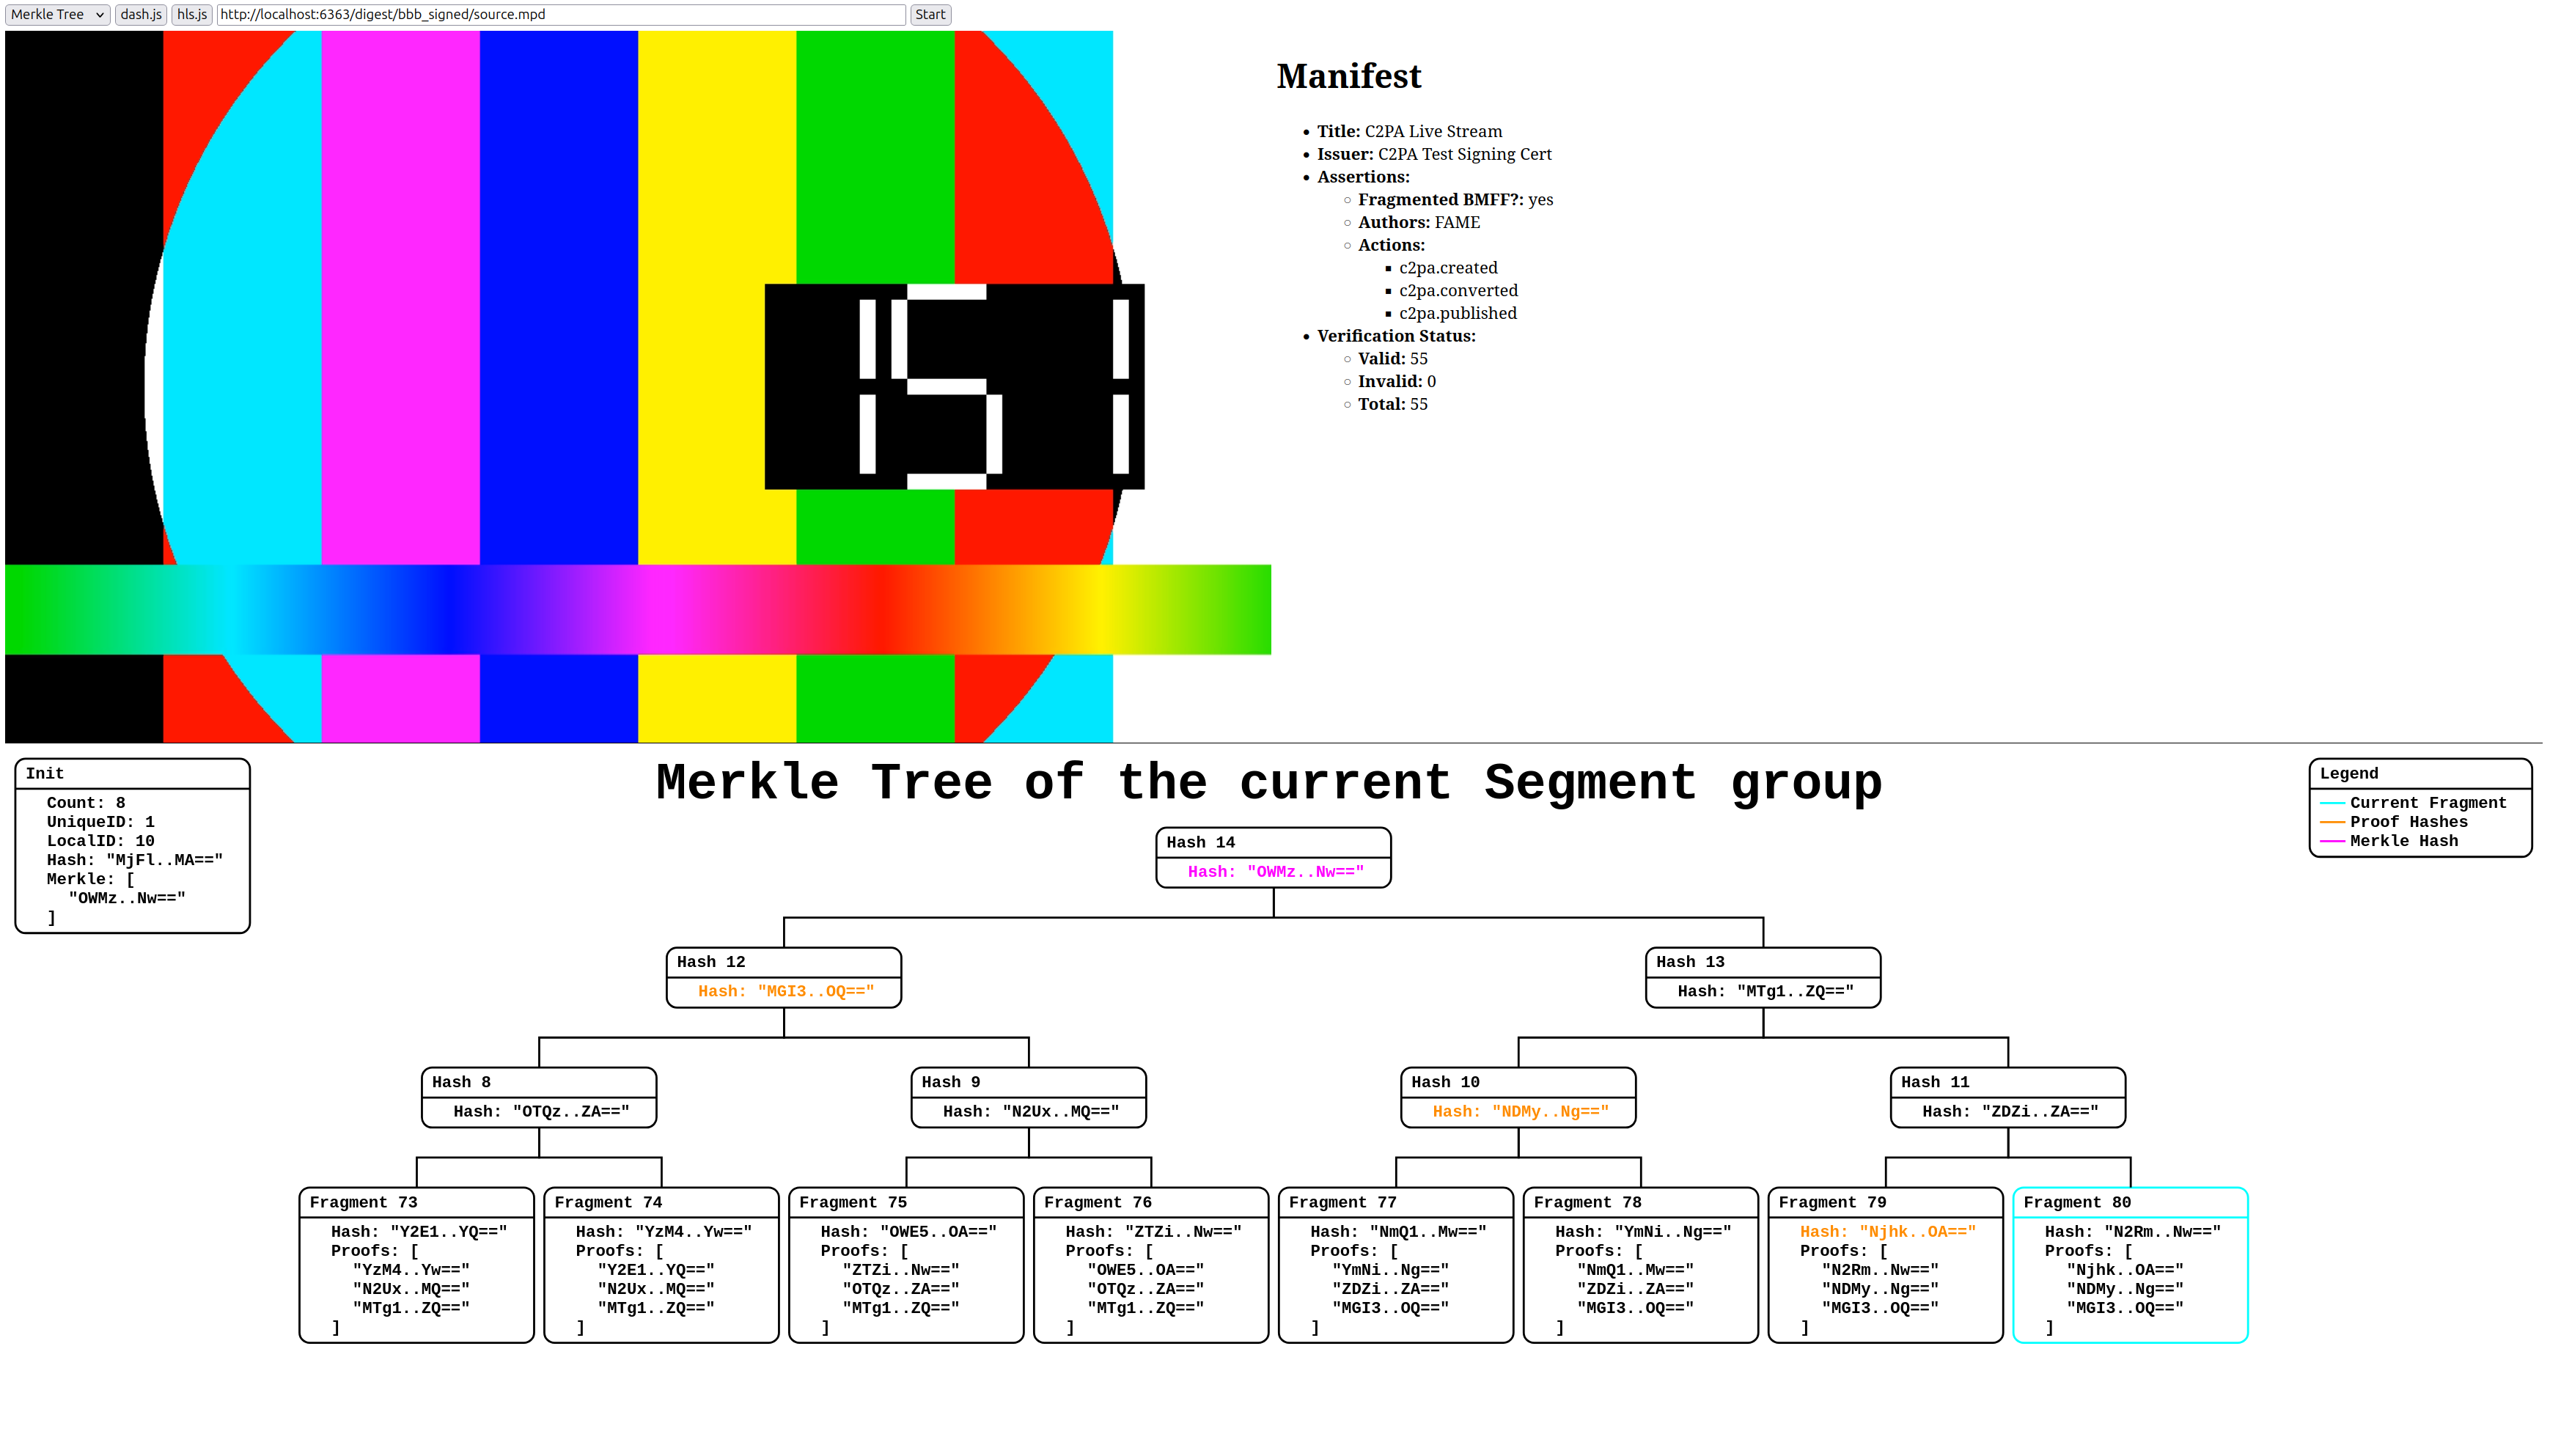
\includegraphics[width=0.95\linewidth, fbox]{merkle-tree-full.png}
    \caption{Example Merkle Tree Visualization}
    \label{fig:merkle_tree}
\end{figure}
\begin{figure}
    \centering
    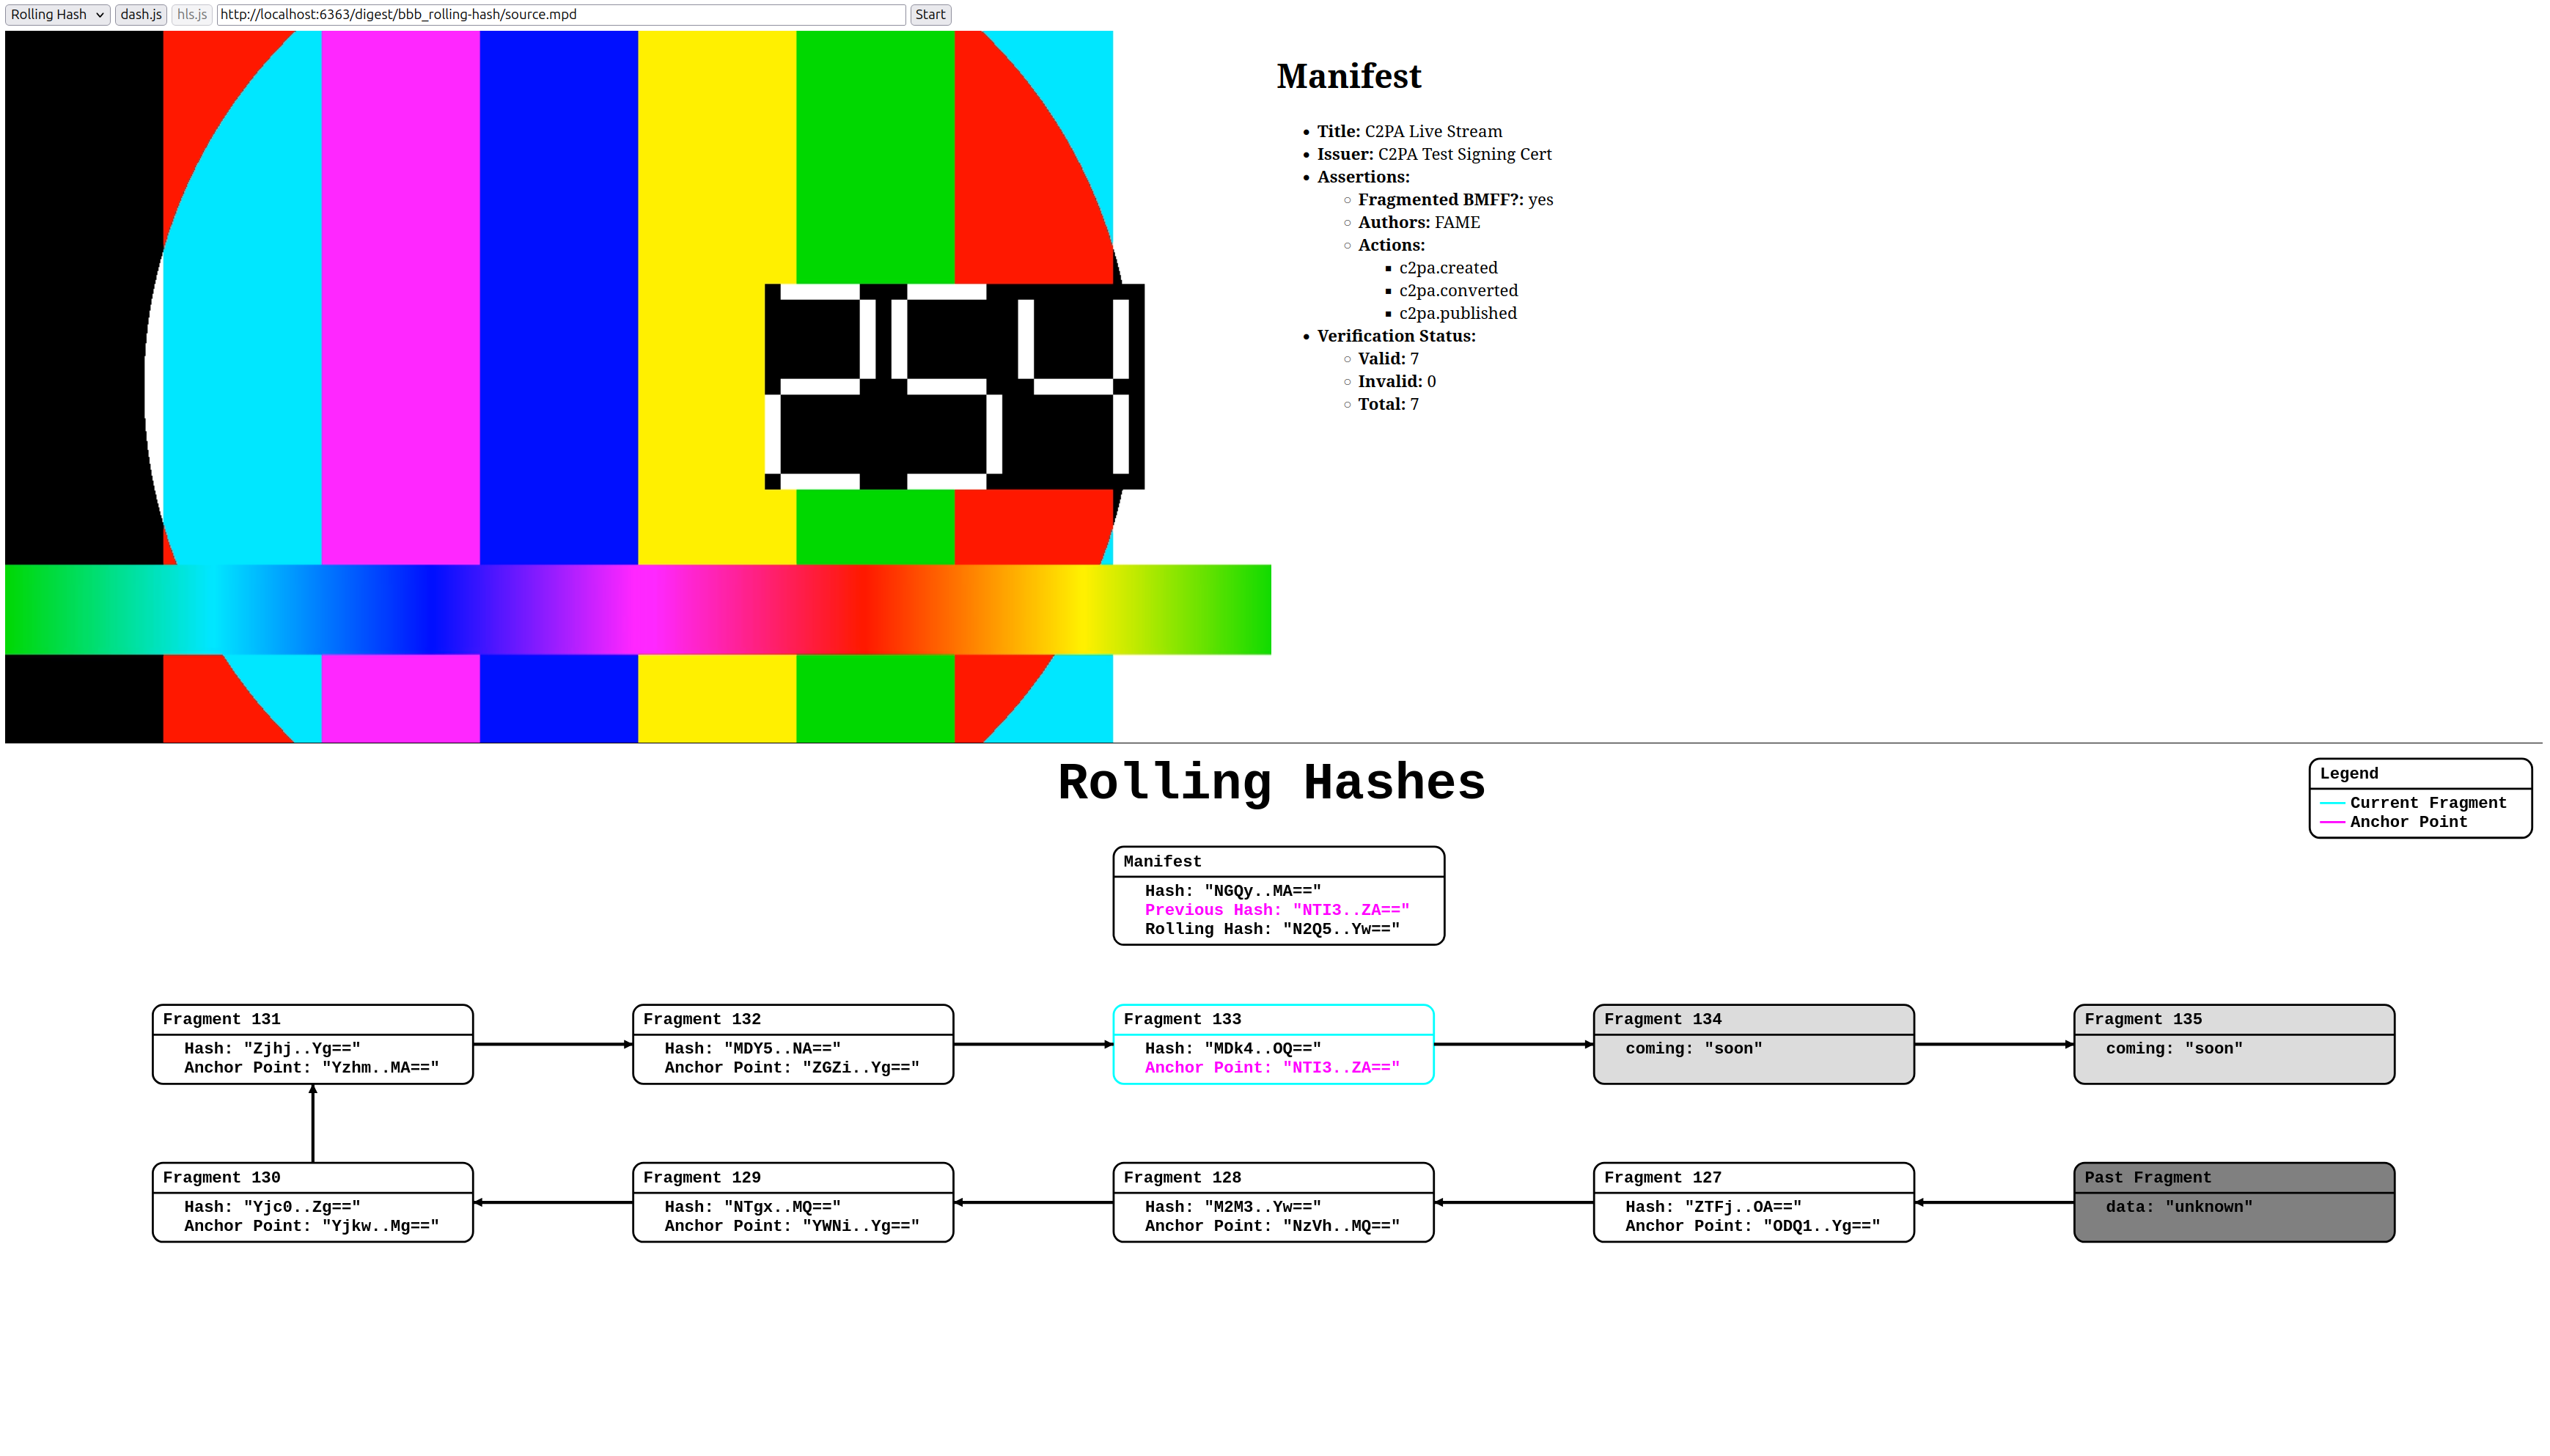
\includegraphics[width=0.95\linewidth, fbox]{rolling-hash.png}
    \caption{Example Rolling Hash Visualization}
    \label{fig:rolling_hash}
\end{figure}

The \textbf{Controls} can be separated into two parts. 

The first being two buttons and a drop down selector for convenience. The buttons are pre-configured to play the signed live stream generated in this testbed using either \texttt{dash.js} or \texttt{hls.js}. The drop down selector allows the choosing of which of the live streams to watch: the unsigned original, the Merkle Tree approach or the Rolling Hash method.

The second part is an URL text input to use any other live stream and a button to start the live stream using that URL. In this case the website will determine which player to use based on the given URL, specifically using the file extension:

\begin{itemize}
    \item "mpd" for \texttt{dash.js}
    \item "m3u8" for \texttt{hls.js}
\end{itemize}

The next component is the \textbf{Player} and this is a standard HTML5 video element. This video element is used by the players to play the live stream. Both players have also been extended using their public event callback APIs to validate the requested media fragments using the aforementioned \texttt{c2pa} JavaScript package. For the Rolling Hash validation, the \texttt{c2pa} has been extended with an API to verify those fragments. Details on this implementation follow in \Cref{sec:wasm}.

The \textbf{Manifest} visualization is third component and is used to display a few selected parts of the C2PA manifest found in the live stream being played. Shown information are the title of the manifest, the issuer of the certificate used to sign the manifest and the assertions: whether it is a fragmented BMFF format, the author of the manifest and all actions applied to the live stream. Finally, I have also used this space to display the current validation status of all fragments by showing the number of valid, invalid and total fragments. In case a fragment is determined to be invalid it will also display the reason why the fragment was invalid.

The final component is the \textbf{Visualization} of the Merkle Tree and Rolling Hash and it dynamically creates SVG images of the current state of the Merkle Tree in form of a binary tree or Rolling Hash as snaking chain of individual hashes. It shows the initialization fragment, the Merkle Tree or Rolling Hash chain and a legend for the colors used. The initialization fragment display contains information of the Merkle Tree referenced by the most recent fragment: the current number of leaves, the unique and local ID, its hash and the reference Merkle Tree hash. The Merkle Tree display shows the reconstructed Merkle Tree based on the current fragment In case of the Rolling Hash the initialization fragment displays its hash and the Rolling Hash and Anchor Point. The leaves (the fragments) list their own data hash and the proof hashes needed for validation. The current fragment is marked by a cyan border. Its proof hashes are colored in orange, in the fragment itself and also in the corresponding node in Merkle Tree. The reference Merkle Tree hashes from the initialization fragment, in this testbed the root node, are colored in magenta. Finally, these colors and their meaning are documented in the legend.
